\documentclass[UTF8]{ctexart}
\usepackage[paper=a4paper,dvips,top=2.5cm,left=2.8cm,right=2.8cm,foot=1cm,bottom=3.2cm]{geometry}
\usepackage{fancyhdr}
\usepackage{indentfirst}
\usepackage{enumerate}
\usepackage{clrscode}
\usepackage{listings}
\usepackage{amsmath}
\usepackage{amstext}
 \thispagestyle{empty} 
\lstset{language=Matlab}%代码语言使用的是matlab
\lstset{breaklines}%自动将长的代码行换行排版
\lstset{extendedchars=false}%解决代码跨页时,章节标题,页眉等汉字不显示的问题
\usepackage{graphicx}
\usepackage[colorlinks,linkcolor=blue,urlcolor = blue]{hyperref}
\DeclareGraphicsExtensions{.eps,.ps,.jpg,.bmp}
\pagestyle{plain}
\begin{document}
\par 王博士,您好
\newline
\par 我仔细阅读了您的这篇论文:“Learning User-Specific Latent Influence and
Susceptibility from Information Cascades”,并对cascade size prediction做了仿真。仿真过程中用到的数据集为train.dat.1、net.1以及source.ret.dat.1(训练和测试均在同一数据集上进行)。仿真结果如图$1$所示,结果并不好。真实数据在cascade size为2处有一个波峰,而预测结果的波峰在1处。同时,MAPE值为1.27,比您论文中的结果0.140大了一个数量级。
\begin{figure}[h!]
    \centering
    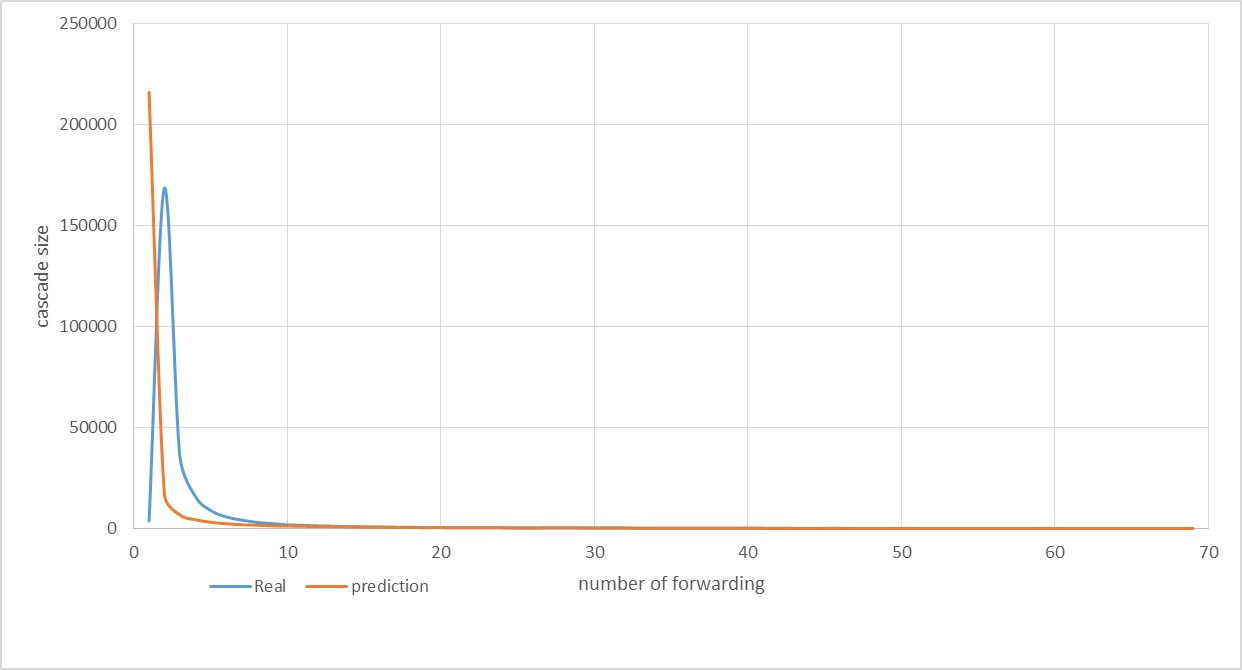
\includegraphics[width=12cm]{cascade.jpg}
    \caption{预测结果}
    \label{fig-sample}
\end{figure}
\par 我有一些疑问,不知您可否帮我解答一下?
\begin{enumerate}[\indent (1)]
    \item 向量$I_{u}$和$S_{v}$是$n$维向量,$n$值应该怎么取?
    \item 在train.dat.1中,某些数据如“1$|$32335*-3349$|$1”中的*号代表什么含义?
    \item 在对目标函数$$\L (C) = -\sum _{v \in V}\sum _{D_{v,i}\in \Gamma (v)}^{N}(n_{z_{v,i},D_{v,i}}log \; p(z_{v,i}\mid z_{v,i-1}, D_{v,i},\delta)) + \gamma _{I}\left \| I \right \|_{F}^{2}+\gamma _{S}\left \| S \right \|_{F}^{2}$$使用投影梯度下降法时,目标函数的初始值大概在$8.6\times 10^{6}$左右,经过几百次的迭代下降后(需要数个小时)也只能下降十分之一。目标函数是凸函数吗?投影梯度下降能找到最优解吗?
    \item 原文公式$9$中的$$\frac{\partial \L}{S_{v}}=-\lambda \sum _{D_{v,i}\in \Gamma (v)}\sum _{u \in D_{v,i}} I _{u}(n_{z_{v,u}=1,D_{v,u}}\frac{1-p_{v,D_{v,u}}}{p_{v,D_{v,u}}}-n_{z_{v,u}=0,D_{v,u}})+\gamma _{S}S_{v} $$中的cascade context为何是$D_{v,u}$而不是$D_{v,i}$呢?
    \item 能否告知我一些参数的值或范围?比如$\lambda$、$\gamma _{I}$、$\gamma _{S}$。
\end{enumerate}
\end{document}
